\chapter{Comparison of the CM with the MCA}

\label{comparison_chapter}

To test and validate the system of differential equations \eqref{general_system} I compare its solutions at different initial and boundary conditions with the results of MCA simulations. In this chapter I first describe the implementations of the CM and the MCA, that are used for the comparison. Second, I discuss the approximations, where the system \eqref{general_system} can be solved numerically, and provide some efficient numerical methods that can be used. Finally, I present the comparison of the CM and the MCA approaches in a number of biophysical situations.

\section{MCA description}

\label{new_MCA_description}

To be able to compare the CM and the MCA models, I modified the MCA by explicit consideration of the diffusion of all lipid species in the membrane (in the CM all lipid species undergo lateral diffusion). However, otherwise the MCA has the same characteristics, described in the chapter \ref{Monte_Carlo_model_description}.

To compute the probability distribution of the peptide on the membrane, the peptide is initially put in the middle of the lattice and then is allowed to undergo $5\cdot10^6$ diffusion steps. The position of the peptide at every step is collected. Using averaging over the lattice size and over the number of iterations the peptide probability distribution is calculated. Additional averaging of the probability distribution over 10 peptide trajectories is also performed. To be able to calculate an energy change corresponding to one peptide movement, the peptide hexagon (dashed line in Fig. \ref{fig:peptide_neighborhood}) is not allowed to approach the lattice boundaries closer than 3 lipid distances.

\section{General solution of the CM using FlexPDE}

\label{FlexPDE_description}

To solve the general system of membrane dynamics equations \eqref{general_system} I take advantage of a commercial software FlexPDE, which is often used for obtaining numerical solutions to partial differential equations. It is based on the Finite Element Method \cite{Zienkiewicz2005}.

In the general case the system \eqref{general_system} should be solved in a 2D membrane domain. However, since the lipid and peptide distributions in the MCA can be averaged along one dimension, the MCA can be considered as a 1D system. Therefore, for simplicity, in the CM I solve the system \eqref{general_system} in 1D. However, in the other situations (when the lipid and the peptide profiles in the MCA are more complicated) solution of the system \eqref{general_system} has to be obtained in 2D.

To adjust an accuracy of the solution I define the following parameters required by FlexPDE:

\begin{enumerate}
 \item Tolerance: ERRLIM = 0.001 (default value);
 \item Number of mesh points: NGRID = 100 (initial value) -- FlexPDE adjusts it automatically during the calculation;
\end{enumerate}

Boundary conditions are defined explicitly in FlexPDE. In the CM I use two types of boundary conditions: zero flux boundary condition (corresponding to the zero flux of a particular species through the boundary) or fixed value boundary conditions (corresponding to a specific value of concentration at the boundary). 

The CM equivalent of the lipid production rate in the MCA are the interconversion terms (LIIs) introduced in subsection \ref{source_terms}. In FlexPDE the interconversion is created by means of a smooth step function (SWAGE) at one of the membrane boundaries.

\section{Numerical solution of the simplified CM}

\label{numerical_solution}

In the case of small concentrations of negatively charged lipids ($c_i\ll C_m$) or in the case of binary membrane (with neutral and charged species) when the diffusion of only charged lipids is explicitly considered, the general system of membrane equations \eqref{general_system} can be reduced to the system of Poisson-Boltzmann-Nernst-Planck equations (see subsection \ref{lipid_simplification}):
\begin{align}
\label{general_system_simplified}
\frac{\partial c_i}{\partial t}&=\vec{\mathbf{\nabla}} \Big(D_i\Big[\vec{\mathbf{\nabla}} c_i + z_i c_i \vec{\mathbf{\nabla}}\psi \Big]\Big) + K_{i} \nonumber \\
\frac{\partial p_{0,j}}{\partial t}&=\vec{\mathbf{\nabla}} \Big(D_{0,j}\Big[\vec{\mathbf{\nabla}} p_{0,j} + \Big(z_{0,j} + (5 - z_{0,j})\frac{c_1}{C_m}\Big) p_{0,j} \vec{\mathbf{\nabla}}\psi\Big]\Big) + R_{0,j}^p \nonumber \\
\vec{\mathbf{\nabla}}^2 \psi&=\frac{1}{\lambda^2}\sinh(\psi) - \frac{e^2 N_A}{k_B T\varepsilon\varepsilon_0} \sum_{i=1}^3 z_i c_i - \frac{e^2 N_A}{k_B T\varepsilon\varepsilon_0} \sum_{j=0}^5 z_{0,j} p_{0,j}
\end{align}

This system can be solved numerically using known computational techniques. Below I describe some efficient methods that can be used to solve it. I will describe numerical methods of solution of \eqref{general_system_simplified} in a more general 2D case, but if necessary they can be easily simplified to a 1D case.

In the numerical solution of \eqref{general_system} assumptions \eqref{peptide_assumption1} and \eqref{peptide_assumption2} are also used to exclude the impact of the PLCs to the PS membrane concentration.

\subsection{Quasi steady state approximation}

\label{quasi_steady_state}

To choose a numerical method of solution of eqs. \eqref{general_system_simplified} it is necessary to estimate characteristic diffusion and reaction times of the system. If characteristic reaction times are much shorter than diffusion times, it is possible to separate the solution of reaction terms $K_{i}$ and $R_{0,j}^p$ from the solution of diffusion terms and use an explicit method of solution. Otherwise, an implicit method should be used. As $K_1$ and $K_2$ are the constant LIIs, they do not depend on the concentration of any component in the system and can be separated from the diffusion part of the first equation in \eqref{general_system_simplified}.

The characteristic diffusion time in 2D can be estimated as follows:
\begin{equation}
 \tau_D = \frac{L^2}{4D}
\end{equation}
where $L$ is the characteristic size of the membrane domain and $D$ is the diffusion coefficient of the membrane species. Using the following values: $L\sim 100$ nm and $D$=1 $\mu$m$^2$/s, I estimate the characteristic diffusion time as
\begin{equation}
 \tau_D\approx10^{-3} \hspace{0.08in} \text{s}
\end{equation}

Characteristic times of peptide transition reactions $R_{0,j}^p$ can be estimated using the values of the transition reaction constants \eqref{electro_reaction_constants}:
\begin{equation}
 \tau_R \sim \frac{1}{k_{PS} c_1} \approx \frac{1}{h_{PS}} = 10^{-6} \hspace{0.08in} \text{s}
\end{equation}

Comparing two characteristic times one can conclude:
\begin{equation}
 \label{quasi_steady_state_approximation}
\tau_D \gg \tau_R
\end{equation}

Condition \eqref{quasi_steady_state_approximation} means that the peptide diffusion and the peptide transition reactions occur on different time scales. Based on this fact, one can assume that the peptide transition reactions are always equilibrated (a quasi steady state approximation), regardless of the state of the PLCs, and their solution can be separated from the solution of the diffusion part of the peptide equation in \eqref{general_system_simplified}. Thus, an explicit numerical method can be used to obtain the solution.

\subsection{Analytical solution of peptide transition reactions}

\label{analytical_electro_reaction}

In the quasi steady state approximation (with assumptions \eqref{peptide_assumption1} and \eqref{peptide_assumption2}) described above the system of peptide transition reactions \eqref{er_p00}--\eqref{er_p05} can be solved (for its steady state) at every diffusion step. Mathematically, at the steady-state time derivatives of all components become 0. The steady state solution of the peptide transition equations \eqref{er_p00}--\eqref{er_p05} has the following form:
\begin{equation}
 \label{peptide_steady_state}R_{0,j}^p = 0,\hspace{0.1in} j\in[0;5]
\end{equation}

System \eqref{peptide_steady_state} can be solved analytically:

\begin{equation}
 \label {p01} p_{0,1} = \frac{k_{0,0}}{h_{0,1}}\cdot p_{0,0} \cdot c_1 = A_{0,1}\cdot p_{0,0} \cdot c_1
\end{equation}
\begin{equation}
 \label {p02} p_{0,2} = \frac{k_{0,0}k_{0,1}}{h_{0,1}h_{0,2}}\cdot p_{0,0} \cdot c_1^2 = A_{0,2}\cdot p_{0,0} \cdot c_1^2
\end{equation}
\begin{equation}
 \label {p03} p_{0,3} = \frac{k_{0,0}k_{0,1}k_{0,2}}{h_{0,1}h_{0,2}h_{0,3}}\cdot p_{0,0} \cdot c_1^3 = A_{0,3}\cdot p_{0,0} \cdot c_1^3
\end{equation}
\begin{equation}
 \label {p04} p_{0,4} = \frac{k_{0,0}k_{0,1}k_{0,2}k_{0,3}}{h_{0,1}h_{0,2}h_{0,3}h_{0,4}}\cdot p_{0,0} \cdot c_1^4 = A_{0,4}\cdot p_{0,0} \cdot c_1^4
\end{equation}
\begin{equation}
 \label {p05} p_{0,5} = \frac{k_{0,0}k_{0,1}k_{0,2}k_{0,3}k_{0,4}}{h_{0,1}h_{0,2}h_{0,3}h_{0,4}h_{0,5}}\cdot p_{0,0} \cdot c_1^5 = A_{0,5}\cdot p_{0,0} \cdot c_1^5
\end{equation}

In the system \eqref{p01}--\eqref{p05} concentrations of all PLCs are defined by means of the concentration of the free peptide, $p_{0,0}$, and the concentration of PS lipids, $c_1$. Thus, one can avoid the solution of all peptide equations in the system \eqref{general_system_simplified}, except $p_{0,0}$, and find concentrations of other PLCs using eqs. \eqref{p01}--\eqref{p05}.

\subsection{Discretization of Nernst-Planck equation}

\label{nernst_planck_discretization}

As described in subsection \ref{quasi_steady_state}, diffusion and reaction terms in the first two equation of the system \eqref{general_system_simplified} can be separately solved and explicit numerical method can be used to find the solution of the diffusion part. In this section I describe an efficient method of solution of the diffusion (Nernst-Planck) parts of these equations. First, I rewrite them in the following general form:
\begin{equation}
\frac{\partial c}{\partial t}=\vec{\mathbf{\nabla}}[D(\vec{\mathbf{\nabla}} c+z c\vec{\mathbf{\nabla}} \psi)]
\end{equation}
where $c$, $D$ and $z$ are correspondingly the concentration, the diffusion coefficient and the charge of any membrane species (lipids or peptides); $\psi$ is the electrostatic potential. This equation represents a class of advection-diffusion equations and can be rewritten in the following form:
\begin{align}
\label{ADE}
\frac{\partial c}{\partial t}&=\vec{\mathbf{\nabla}} (D\vec{\mathbf{\nabla}} c)-\vec{\mathbf{\nabla}} (c \vec{\mathbf{v}}) \nonumber \\
 \vec{\mathbf{v}} &= - D z \vec{\mathbf{\nabla}} \psi
\end{align}

To solve these equations numerically I use a novel explicit, accurate and efficient discretization scheme (``master equation discretization'' or MED) proposed by R. Grima and T.J. Newman \cite{Grima2004}. They have shown that this scheme is more accurate than commonly used simple Taylor expansion or the ``upwind'' schemes. They derive a general discretized form of eq. \eqref{ADE} in 1D (it can be used for solution of \eqref{general_system_simplified} in 1D). I use the same procedure to derive a discretized form of equation \eqref{ADE} in 2D. To obtain a general form of the equation suitable for MED one has to define two scalar functions $f$ and $g$ as follows:
\begin{align}
\label{D}
D &= f g \nonumber \\
\vec{\mathbf{v}} &= g \vec{\mathbf{\nabla}} f - f \vec{\mathbf{\nabla}} g
\end{align}

If functions \(f\) and \(g\) are defined by \eqref{D}, then, by direct differentiation, one can show that eq. \eqref{ADE} can be rewritten as:
\begin{equation}
\label{suitable_MED}
\frac{\partial c}{\partial t} = f \vec{\mathbf{\nabla}}^2(g c) - gc \vec{\mathbf{\nabla}}^2 f
\end{equation}

To satisfy the eqs. \eqref{D}, the functions $f$ and $g$ can be chosen as follows:
\begin{align}
\label{f}
f&=D \exp(-\frac{z}{2}\psi) \\
\label{g}
g&=\exp(\frac{z}{2}\psi)
\end{align}

If the membrane is a square mesh with the size of $N$ nodes and spatial resolution $h$, then all functions in equation \eqref{suitable_MED} can be projected on it (on the mesh). Using the five-point discretization scheme shown in Fig. \ref{fig:computational_scheme}, one can obtain the discretized form of equation \eqref{suitable_MED} on the mesh:
\begin{align}
\label{discrete1}
\frac{c_{m,n}^{t+1} - c_{m,n}^{t}}{\tau} &= \nonumber \\
&= f_{m,n}^{t}\Big[ \frac{g_{m-1,n}^{t} c_{m-1,n}^{t} + g_{m+1,n}^{t} c_{m+1,n}^{t}}{h^2} + \nonumber \\
 &+ \frac{g_{m,n-1}^{t} c_{m,n-1}^{t} + g_{m,n+1}^{t} c_{m,n+1}^{t} - 4 g_{m,n}^{t} c_{m,n}^{t}}{h^2}\Big]- \nonumber \\
&- g_{m,n}^{t} c_{m,n}^{t} \frac{f_{m-1,n}^{t} + f_{m+1,n}^{t} + f_{m,n-1}^{t} + f_{m,n+1}^{t} - 4 f_{m,n}^{t}}{h^2}
\end{align}

\begin{figure}[!ht]
\centering
  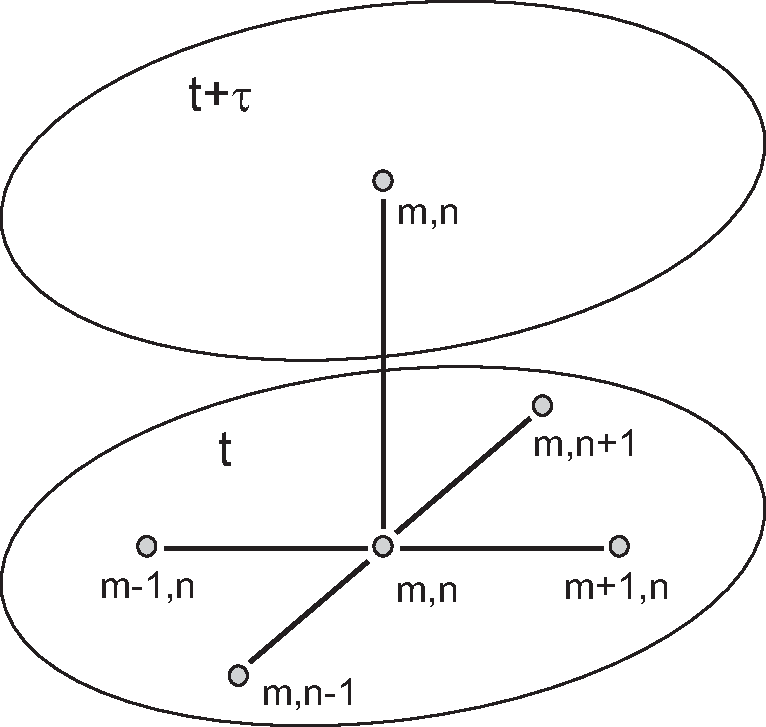
\includegraphics[scale=0.5]{../figures/scheme.pdf}
\caption[Numerical five-point scheme used in MED method]{Numerical five-point scheme used in MED method. Five known points on the level $t$ are used to calculate a new point on level $t+\tau$.}
\label{fig:computational_scheme}
\end{figure}

Equation \eqref{discrete1} can be simplified to:
\begin{align}
\label{discrete2}
&c_{m,n}^{t+1} - c_{m,n}^{t} = \nonumber \\
&= \frac{\tau}{h^2} \bigg[ c_{m-1,n}^{t} (f_{m,n}^{t} g_{m-1,n}^{t})  + c_{m+1,n}^{t} (f_{m,n}^{t} g_{m+1,n}^{t}) + \nonumber \\ 
&+ c_{m,n-1}^{t}(f_{m,n}^{t} g_{m,n-1}^{t}) + c_{m,n+1}^{t} (f_{m,n}^{t} g_{m,n+1}^{t})  - \nonumber \\
&- c_{m,n}^{t} g_{m,n}^{t} (f_{m-1,n}^{t} + f_{m+1,n}^{t} + f_{m,n-1}^{t} + f_{m,n+1}^{t}) \bigg]
\end{align}


Substituting functions $f$ and $g$ into equation \eqref{discrete2}, one can obtain the final form of the discretized equation: 
\begin{align}
\label{discrete_final}
&c_{m,n}^{t+1} - c_{m,n}^{t} = \nonumber \\
&= \frac{D\tau}{h^2} \bigg[ c_{m-1,n}^{t} \exp(-\frac{z}{2}(\psi_{m,n}^{t} - \psi_{m-1,n}^{t}))  + c_{m+1,n}^{t} \exp(-\frac{z}{2}(\psi_{m,n}^{t} - \psi_{m+1,n}^{t})) + \nonumber \\ 
&+ c_{m,n-1}^{t} \exp(-\frac{z}{2}(\psi_{m,n}^{t} - \psi_{m,n-1}^{t})) + c_{m,n+1}^{t} \exp(-\frac{z}{2}(\psi_{m,n}^{t} - \psi_{m,n+1}^{t}))  - \nonumber \\
&- c_{m,n}^{t} \bigg(\exp(-\frac{z}{2}(\psi_{m-1,n}^{t} - \psi_{m,n}^{t})) + \exp(-\frac{z}{2}(\psi_{m+1,n}^{t} - \psi_{m,n}^{t})) + \nonumber \\ 
&+ \exp(-\frac{z}{2}(\psi_{m,n-1}^{t} - \psi_{m,n}^{t})) + \exp(-\frac{z}{2}(\psi_{m,n+1}^{t} - \psi_{m,n}^{t}))\bigg) \bigg]
\end{align}

Using an iterative procedure this discretized equation can be used to find a solution of the original eq. \eqref{ADE}. I have tested this discretization scheme in 2D and it was stable and accurate in the reasonable range of time steps and mesh units, allowing to efficiently compute the solution of eq. \eqref{ADE}.

\subsection{Discretization of Poisson-Boltzmann equation}

The last equation in the system \eqref{general_system_simplified} is the Poisson-Boltzmann equation. To solve this equation computationally I use Newton-Raphson iterative method \cite{Carnie1994,Harries1998}, which has been shown to be accurate and efficient in solutions of different types of equations. This method works as follows. Assume that the following equation, which is equivalent to Poisson-Boltzmann equation in \eqref{general_system_simplified} has to be solved:
\begin{equation}
 \label{poisson-boltzmann_newt-raphs0}\Delta\psi = A \sinh{\psi} - f(c)
\end{equation}
where $\psi$ is the electrostatic potential, $A$ is a constant and $f(c)$ is a function of concentrations of system components. One can define an iterative process of finding a solution of eq. \eqref{poisson-boltzmann_newt-raphs0} as:
\begin{equation}
 \label{delta_psi_def}\psi^{l+1} = \psi^l + \delta \psi
\end{equation}
where $\psi^{l+1}$ is an approximate solution of eq. \eqref{poisson-boltzmann_newt-raphs0} on $(l+1)$ iteration and $\delta \psi$ is an increment of the previous estimate of the solution $\psi^l$. Substitution of \eqref{delta_psi_def} to \eqref{poisson-boltzmann_newt-raphs0} provides:
\begin{equation}
 \label{poisson-boltzmann_newt-raphs1}\Delta\psi^l + \Delta(\delta\psi) = A \sinh{(\psi^l+\delta\psi)} - f(c)
\end{equation}

For a small $\delta\psi$, $\sinh(\psi^l)$ can be linearized as follows:
\begin{equation}
 \sinh(\psi^l+\delta\psi) = \sinh(\psi^l) + \sinh'(\psi^l)\delta\psi
\end{equation}

Taking into account that $\sinh'(\psi^l) = \cosh(\psi^l)$, one can derive:
\begin{equation}
 \label{poisson-boltzmann_newt-raphs2}\Delta\psi^l + \Delta(\delta\psi) = A\sinh(\psi^l) + A\cosh(\psi^l)\delta\psi - f(c)
\end{equation}

Rearranging of eq. \eqref{poisson-boltzmann_newt-raphs2} and utilizing eq. \eqref{delta_psi_def}, one can obtain a general form of Newton-Raphson iterations for solution of the Poisson-Boltzmann equation:
\begin{equation}
 \label{poisson-boltzmann_newt-raphs3}\Delta\psi^{l+1} - A\psi^{l+1}\cosh(\psi^l)  = A\sinh(\psi^l) - A\psi^l\cosh(\psi^l) - f(c)
\end{equation}

The original equation \eqref{poisson-boltzmann_newt-raphs0} is now reduced to a solution of a sequence of linear elliptic equations \eqref{poisson-boltzmann_newt-raphs3}. Considering the same lattice as used in the solution of Nernst-Planck equation (see subsection \ref{nernst_planck_discretization}) and the same discretization scheme (Fig. \ref{fig:computational_scheme}), one can define a discretized form of eq. \eqref{poisson-boltzmann_newt-raphs3} in 2D space:
\begin{align}
 \label{poisson-boltzmann_newt-raphs4}&\psi^{l+1}_{m+1,n}+\psi^{l+1}_{m-1,n}+\psi^{l+1}_{m,n+1}+\psi^{l+1}_{m,n-1}-(4+h^2A\cosh(\psi^l_{m,n}))\psi^{l+1}_{m,n} = \nonumber \\
 &=h^2A\sinh(\psi^l_{m,n}) - h^2A\psi^l\cosh(\psi^l_{m,n}) - h^2f(c) 
\end{align}

Simplification of eq. \eqref{poisson-boltzmann_newt-raphs4} yields:
\begin{equation}
  \label{poisson-boltzmann_newt-raphs5}\psi^{l+1}_{m+1,n}+\psi^{l+1}_{m-1,n}+\psi^{l+1}_{m,n+1}+\psi^{l+1}_{m,n-1}+d_{m,n}\psi^{l+1}_{m,n} = e_{m,n} 
\end{equation}

where 
\begin{align}
\label{newton-raphson_coefficients}
 d_{m,n} &= -(4+h^2A\cosh(\psi^l_{m,n})) \nonumber \\
 e_{m,n} &= h^2A\sinh(\psi^l_{m,n}) - h^2A\psi^l\cosh(\psi^l_{m,n}) - h^2f(c)
\end{align}

Coefficients \eqref{newton-raphson_coefficients} are defined by means of known values of $\psi^l_{m,n}$ and $f(c)$. In order to solve eq. \eqref{poisson-boltzmann_newt-raphs5}, one should rewrite it in an extended vector form:
\begin{equation}
  \label{matrix}\begin{pmatrix}
  b_1 & c_1 & 0 & 0 & \cdots & 0 & 0 & a_1 \\
  a_2 & b_2 & c_2 & 0 & \cdots & 0 & 0 & 0 \\
  0 & a_3 & b_3 & c_3 & \cdots & 0 & 0 & 0 \\
  \vdots  & \vdots & \vdots & \vdots  & \ddots & \vdots & \vdots & \vdots  \\
  0 & 0 & 0 & 0 & \cdots& a_{N-1} & b_{N-1} & c_{N-1} \\
  c_N & 0 & 0 & 0 & \cdots & 0 & a_N & b_N
 \end{pmatrix}\times
\begin{pmatrix}
  \vec{\psi_1} \\
  \vec{\psi_2} \\
  \vec{\psi_3} \\
  \vdots \\
  \vec{\psi_{N-1}} \\
  \vec{\psi_N}
 \end{pmatrix} = 
\begin{pmatrix}
  \vec{g_1} \\
  \vec{g_2} \\
  \vec{g_3} \\
  \vdots \\
  \vec{g_{N-1}} \\
  \vec{g_{N}}
 \end{pmatrix}
\end{equation}
where $a_i$, $b_i$ and $c_i$ are matrices of sizes $N\times N$; $\vec{\psi_i}$ and $\vec{g_i}$ are vectors of sizes $N$; $N$ is a number of nodes in the discretized lattice. The forms of matrices $a_i$, $b_i$, $c_i$ and vectors $\vec{\psi_i}$, $\vec{g_i}$ depend on the boundary conditions imposed on the membrane system. In the general case of periodic boundary conditions at every boundary of the membrane, the matrices and vectors have the following structures:
\begin{equation}
 a_i=c_i=
 \begin{pmatrix}
  1 & 0 & 0 & \cdots & 0 & 0 \\
  0 & 1 & 0 & \cdots & 0 & 0 \\
  0 & 0 & 1 & \cdots & 0 & 0 \\
  \vdots  & \vdots & \vdots  & \ddots &  \vdots & \vdots  \\
  0 & 0 & 0 & \cdots & 1 & 0 \\
  0 & 0 & 0 & \cdots & 0 & 1
 \end{pmatrix} = I
\end{equation}
\begin{equation}
 b_i=
 \begin{pmatrix}
  d_{i,1} & 1 & 0 & 0 & \cdots & 0 & 0 & 1 \\
  1 & d_{i,2} & 1 & 0 & \cdots & 0 & 0 & 0 \\
  0 & 1 & d_{i,3} & 1 & \cdots & 0 & 0 & 0 \\
  \vdots  & \vdots & \vdots & \vdots  & \ddots & \vdots & \vdots & \vdots  \\
  0 & 0 & 0 & 0 & \cdots & 1 & d_{i,N-1} & 1 \\
  1 & 0 & 0 & 0 & \cdots & 0 & 1 & d_{i,N}
 \end{pmatrix}
\end{equation}
\begin{equation}
 \vec{\psi_i}=
 \begin{pmatrix}
  \psi^{l+1}_{i, 1} \\
  \psi^{l+1}_{i, 2} \\
  \psi^{l+1}_{i, 3} \\
  \vdots \\
  \psi^{l+1}_{i, N-1} \\
  \psi^{l+1}_{i, N}
 \end{pmatrix};
\hspace{0.2in}
\vec{g_i}=
 \begin{pmatrix}
  e_{i,1} \\
  e_{i,2} \\
  e_{i,3} \\
  \vdots \\
  e_{i,N-1} \\
  e_{i,N}
 \end{pmatrix}
\end{equation}

If one defines a matrix on the left hand side of eq. \eqref{matrix} as $M$, then solution of eq. \eqref{matrix} can be explicitly derived as follows:
\begin{equation}
\label{matrix1}
\begin{pmatrix}
  \vec{\psi_1} \\
  \vec{\psi_2} \\
  \vec{\psi_3} \\
  \vdots \\
  \vec{\psi_{N-1}} \\
  \vec{\psi_N}
 \end{pmatrix} = M^{-1}
\begin{pmatrix}
  \vec{g_1} \\
  \vec{g_2} \\
  \vec{g_3} \\
  \vdots \\
  \vec{g_{N-1}} \\
  \vec{g_{N}}
 \end{pmatrix}
\end{equation}

This means that, to find the electrostatic potential in every point of the membrane at ($l+1$) iteration, it is necessary to invert the matrix $M$ and multiply it with the vector $\vec{g}$. Notice that both these values (on the right hand side of eq. \eqref{matrix1}) are known and explicitly defined through the values of $d_{m,n}$ and $e_{m,n}$ \eqref{newton-raphson_coefficients}.

Before reaching a steady state regime lipid and PLCs concentration profiles change with time. Consequently the electrostatic potential has to be constantly updated (it is created by the charged lipids and PLCs), i.e. Poisson-Boltzmann equation (or the inversion of the matrix $M$) has to be solved at every diffusion step. Thus, the complexity of the matrix inversion algorithm, used in the solution of Poisson-Boltzmann equation, is an important parameter, which defines the effectiveness of the total numerical method of solution of \eqref{general_system_simplified}. Since the size of $M$ is $N^2\times N^2$, the numerical complexity of the general inversion procedure varies from $O(N^{4.5})$ to $O(N^6)$, depending on the algorithm. However, due to a specific structure of $M$ (periodic block-tridiagonal) it is possible to reduce the complexity of the inversion to about $O(N^{3.5})$--$O(N^4)$, by applying algorithms developed for matrices with such structure \cite{Napolitano1985,Bieniasz2001}. This complexity is minimal to obtain an exact analytical solution of eq. \eqref{matrix}, however it is still computationally inefficient. To further reduce a complexity of matrix inversion the following simplified method can be used. Namely, instead of the general matrix inversion in 2D, the inversion in 1D (vertical columns or horizontal lines of the mesh) can be performed $N$ times. The reduction of the system from 2D to 1D can be done by assuming that two values of the electrostatic potential in eq. \eqref{poisson-boltzmann_newt-raphs5} at $(l+1)^{\text{th}}$ iteration are known and equal to the values of the potential at $l^{\text{th}}$ iteration (see Fig. \ref{fig:computational_scheme1}). Under this assumption eq. \eqref{poisson-boltzmann_newt-raphs5} transforms to the following form:
\begin{equation}
  \label{poisson-boltzmann_newt-raphs6}\psi^{l+1}_{m,n+1}+\psi^{l+1}_{m,n-1}+d_{m,n}\psi^{l+1}_{m,n} = e^*_{m,n} 
\end{equation}
where 
\begin{align}
\label{newton-raphson_coefficients1}
 d_{m,n} &= -(4+h^2A\cosh(\psi^l_{m,n})) \nonumber \\
 e^*_{m,n} &= h^2A\sinh(\psi^l_{m,n}) - h^2A\psi^l\cosh(\psi^l_{m,n}) - h^2f(c) - (\psi^{l}_{m-1,n} + \psi^{l}_{m,n})
\end{align}

\begin{figure}[!ht]
\centering
  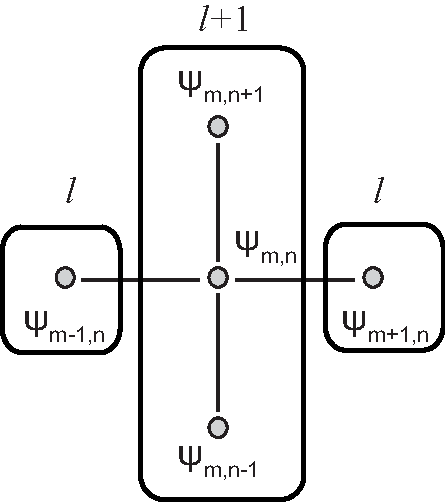
\includegraphics[scale=0.6]{../figures/scheme1.pdf}

\caption[Dimension reduction in the general form of the discretized Poisson-Boltzmann equation]{Dimension reduction in the general form of the discretized Poisson-Boltzmann equation. Two values of potential $\psi_{m-1,n}$ and $\psi_{m+1,n}$ are assumed to be known and equal the values of potential at the previous iteration. Three unknown values $\psi_{m,n-1}$, $\psi_{m,n}$ and $\psi_{m,n+1}$ then can be found at the next iteration in the reduced 1D dimension.}
\label{fig:computational_scheme1}
\end{figure}

The advantage of system \eqref{poisson-boltzmann_newt-raphs6}--\eqref{newton-raphson_coefficients1} over system \eqref{poisson-boltzmann_newt-raphs5}--\eqref{newton-raphson_coefficients} is that it has a reduced dimensional space -- 1D. Matrix $M'$ which has to be inverted in 1D case has a similar structure as matrix $M$ in 2D, except its size is $N\times N$ and instead of matrices $a_i$, $b_i$ and $c_i$ it has parameters $a^*_i$, $b^*_i$ and $c^*_i$ with the following values:
\begin{equation}
 a^*_i = c^*_i = 1; \hspace{0.2in} b^*_i = d_{m,i} (\text{or } d_{i,n} \text{, depending on the algorithm})
\end{equation}

In a general form (with periodic boundary conditions) the matrix $M'$ is a periodic tridiagonal matrix. Inversion of this matrix can be done using a very efficient Thomas algorithm \cite{Conte1980}, the complexity of which is about $O(N)$. However, in this approximation Poisson-Boltzmann equation has to be solved $N$ times in every row or every column of the lattice (to cover the whole lattice). Thus, the total complexity of this approximation method increases to about $O(N^2)$. However, this is still by one order of magnitude more efficient than calculation of an exact analytical solution in 2D space.

I've tested the stability and the accuracy of the simplified method and observed that it was stable in a large range of spatial mesh resolutions and it converged with accuracy of $10^{-8}$ in about 10 iterations. This method can be used for a solution of Poisson-Boltzmann equation in the system \eqref{general_system_simplified}.

\section{Importance of membrane incompressibility}

To understand how important is the restriction of membrane incompressibility \eqref{restriction2} in the description of the lipid dynamics I compared the steady state solutions of the general system of equations \eqref{general_system} solved in FlexPDE with the simplified PBNP system \eqref{general_system_simplified} (can be either solved in FlexPDE or using the numerical methods described in the section \ref{numerical_solution} above).

\begin{figure}[!ht]
\centering
  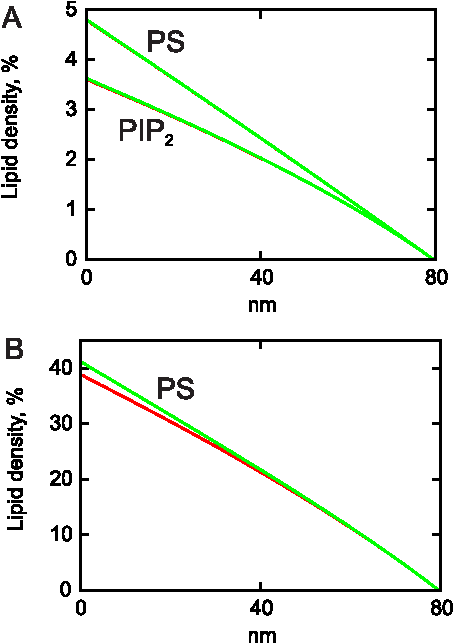
\includegraphics[scale=1.1]{../figures/single_grad_gen_pbnp_comparison.pdf}

\caption[Comparison of general and PBNP systems]{Comparison of general \eqref{general_system} and PBNP \eqref{general_system_simplified} systems. Results of the general system are shown in green, results of the PBNP are shown in red. (A) Small gradients of PS and PIP$_2$; (B) Large gradient of PS.}
\label{fig:single_grad_gen_pbnp_comparison}
\end{figure}

Fig. \ref{fig:single_grad_gen_pbnp_comparison}, A shows that as expected for the dilute concentrations of negatively charged lipids ($<5\%$) discrepancy between two systems \eqref{general_system} and \eqref{general_system_simplified} is negligible and they provide identical results. At higher lipid densities ($\sim 40\%$) the two systems slightly diverge, however, the discrepancy between them is less than 5\% (Fig. \ref{fig:single_grad_gen_pbnp_comparison}, B). Thus, potentially PBNP system can be used to describe the dynamics of lipids in the membrane plane in a large range of concentrations and the membrane incompressibility restriction \eqref{restriction2} can be neglected. However, in the systems with densely packed protein-lipid lattices (or with the protein concentrations comparable to the ones of lipids) this restriction in the extended form (including PLCs -- see subsection \ref{CM_peptide_limitations}) will become more pronounced and should be explicitly taken into account. Therefore, the general system \eqref{general_system} is a more powerful tool (compared to PBNP) which can be further extended to describe systems with different packaging properties.

\section{Results}

\label{continuous_results}

Comparison of the peptide occupations and average total and effective charges on the homogeneous membrane in the CM and in the MCA has already been demonstrated in subsections \ref{reaction_constants} and \ref{total_effective_charge}. In this section I use the solutions of the CM (obtained in FlexPDE) and the MCA to compare the two approaches for the membrane system with a lipid gradient.

First, I calculate the diffusion coefficients of all membrane lipid species in the MCA to utilized them in the CM. I also calibrate the LIIs of lipids, $K_i$ (subsection \ref{source_terms}), in the CM by comparing the two models in the neutral membrane system (the membrane is binary, but both lipid species are neutral). Second, I compare the two models using a single gradient system (the membrane is binary, one lipid species is neutral, the second lipid species is negatively charged, PS or PIP$_2$). Finally, I introduce the peptide species to the system and compare the values of the peptide probability distributions on the membrane.

\subsection{Determination of parameters and calibration of CM}

To determine lipid diffusion coefficients ($D_i$) in the CM, I measure them in the MCA for different membrane compositions. Figs. \ref{fig:neutral_diffusion}, \ref{fig:ps_diffusion} and \ref{fig:pip_diffusion} show the values of $D_i$, normalized by the maximal value of the lipid diffusion coefficient $D_L$ in the uncharged membrane (subsection \ref{testing_calibration_MCA}), for PC, PS and PIP$_2$ lipids, correspondingly. Note different vertical scales in the figures.

\begin{figure}[!ht]
\centering
  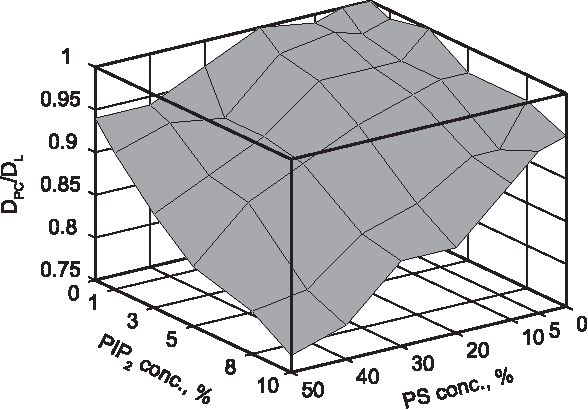
\includegraphics{../figures/neutral_diffusion_no_color.pdf}

\caption[PC diffusion coefficient computed in MCA]{Dependence of PC diffusion coefficient, computed in the MCA, on the membrane composition.}
\label{fig:neutral_diffusion}
\end{figure}

\begin{figure}[!ht]
\centering
  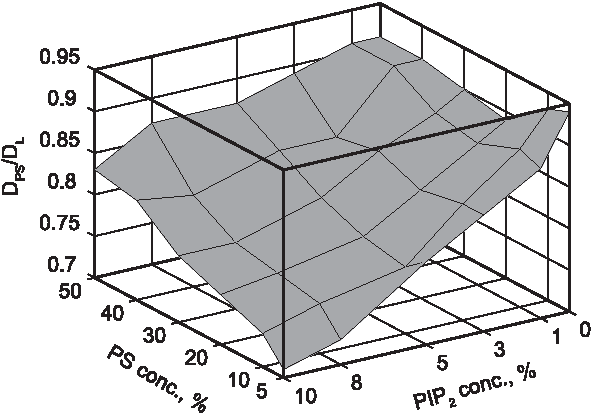
\includegraphics{../figures/ps_diffusion_no_color.pdf}

\caption[PS diffusion coefficient computed in MCA]{Dependence of PS diffusion coefficient, computed in the MCA, on the membrane composition.}
\label{fig:ps_diffusion}
\end{figure}

\begin{figure}[!ht]
\centering
  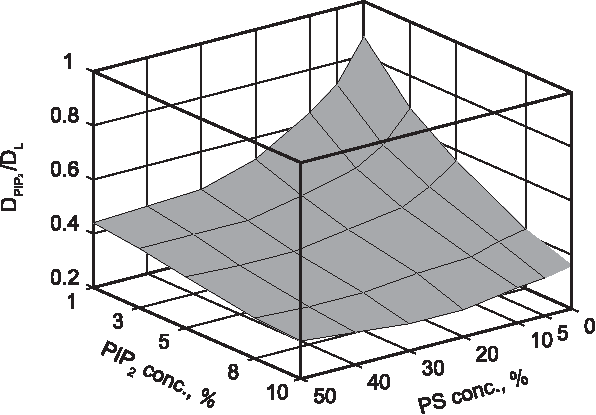
\includegraphics{../figures/pip_diffusion_no_color.pdf}

\caption[PIP$_2$ diffusion coefficient computed in MCA]{Dependence of PIP$_2$ diffusion coefficient, computed in the MCA, on the membrane composition.}
\label{fig:pip_diffusion}
\end{figure}

Since the obtained values of the lipid diffusion coefficients are discrete, in the CM I approximate them as best fits to the functions shown in Figs. \ref{fig:neutral_diffusion}, \ref{fig:ps_diffusion} and \ref{fig:pip_diffusion}. To find the best fit I use polynomic and exponential functions, since FlexPDE software allows one to define complex functions as input parameters. Exact values of the diffusion coefficients that are used in the CM equations are the following:
\begin{equation}
  D_1 (\text{PS}) = D_L\Big(\frac{1}{1+3.5 \tilde{c_1}} + 3\tilde{c_1}\tilde{c_2}\Big)
\end{equation}
\begin{equation}
  D_2 (\text{PIP}_2) = D_L\Big(\frac{1}{1+18 \tilde{c_1}} + 8\tilde{c_1}\tilde{c_2}\Big)(\exp{(-3\tilde{c_2})}+0.5\tilde{c_2})
\end{equation}
\begin{equation}
  D_3 (\text{PC}) = D_L\Big(1 - 3.5\tilde{c_1}\tilde{c_2} - 0.3\tilde{c_1} - 0.1\tilde{c_2}\Big)
\end{equation}
where $\tilde{c_i}$, $i=1,2,3$, are the concentrations of PS, PIP$_2$ and PC, correspondingly, normalized by the total membrane concentration $C_m$.

To calibrate the LIIs, $K_i$, in the CM I consider a system of a binary membrane with two identical neutral (PC) lipid species. A gradient of one species is created by the interconversion of lipids at one boundary. By obtaining the best fit of the CM steady state lipid profiles to the MCA simulation results (Fig. \ref{fig:single_gradient}, A), the LII of neutral lipids, $K_n$, is defined. For the gradient of lipids with 5\% peak value the LII is $K_n=2.34$ M/s ($K^0_1$ hereafter) and for the gradient of lipids with 50\% peak value the LII is $K_n=10 K^0_1 = 23.4$ M/s. The corresponding interconversion rates in the MCA are 0.05 lip/iteration and 0.5 lip/iteration, correspondingly. Thus, in both models, in the case of the neutral membrane system, the peak value of the gradient is directly proportional to the LII. All the values of LIIs, used in the following chapters, lie between $K_1^0$ and $10 K_1^0$.

\subsection{Lipid gradients on binary membrane}
\label{chap:single_gradient}

In this section I describe a comparison of the two approaches on the membrane with a single gradient of negatively charged lipids. Fig. \ref{fig:single_gradient}, B, shows the comparison between the CM and the MCA for a system with a single PS gradient for different values of LIIs. For the small LIIs, $K_1^0$ and $2.5\cdot K_1^0$, when the peak value of the gradient is $<20$\%, the two models provide almost identical results (Fig. \ref{fig:single_gradient}, B and C). However, when the peak value of the gradient is about or more than 20\% one can see an explicit deviation of the CM model from the MCA (Fig. \ref{fig:single_gradient}, B). In the MCA automaton the peak value is always lower and the difference between the models grows with the density of negatively charged lipids. Presumably at high PS densities the mean-field approximations breaks down.
\begin{figure}[!ht]
\centering
  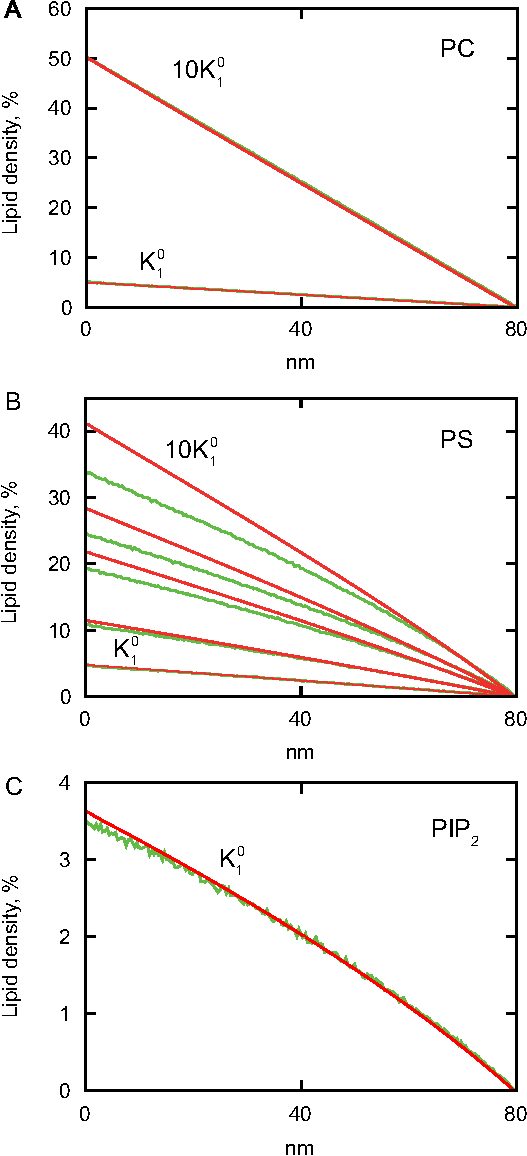
\includegraphics[scale=1.03]{../figures/single_gradient_half_lattice.pdf}

\caption[Comparison of CM and MCA for a single lipid gradient]{Comparison of MCA (green line) and CM (red line) for a single lipid gradient. (A) Gradients of PC in binary PC/PC membrane for two LIIs: $K_1^0$ and $10K_1^0$; (B) Gradients of PS in binary PS/PC membrane for several LIIs: $K_1^0$, $2.5 K_1^0$, $5 K_1^0$, $6.7 K_1^0$ and $10 K_1^0$; (C) A gradient of PIP$_2$ in binary PIP$_2$/PC membrane for the LII $K_1^0$.}
\label{fig:single_gradient}
\end{figure}
The theory that can account for this effect is the so-called strong coupling theory \cite{KanduC2010,Naji2005}. It postulates that highly charged systems are not governed by Poisson-Boltzmann theory (mean-field approximation). Instead, their behavior is better described by the so-called strong coupling limit, where ion-ion correlations are significant. For a system, consisting of a charged surface with a charge density $\sigma$ and a bulk 1:1 electrolyte solution with ion charges $\pm q$ (similar to the membrane system), its regime can be defined using the Netz-Moreira electrostatic coupling parameter, $\Sigma$. This parameter represents a ratio between two characteristic length scales, the Bjerrum length (a typical distance at which two ions $q$ interact with energy $k_BT$, see also eq. \eqref{bjerrum_length0}):

\begin{equation}
\label{bjerrum_length}
 l_B=\frac{e^2}{4\pi\varepsilon\varepsilon_0 k_BT}
\end{equation}
where $e$ is the electron charge, $\varepsilon$ is the dielectric constant of the medium and $\varepsilon_0$ is the vacuum permittivity, and the Gouy-Chapman length (a typical distance at which a counterion $q$ interacts with a charge surface $\sigma$):
\begin{equation}
\label{gouy_chapman_length}
 \mu_{GC} = \frac{e}{2\pi q l_B \sigma}
\end{equation}

So that $\Sigma$ is defined as follows:
\begin{equation}
\label{sigma_coupling_parameter}
 \Sigma = \frac{q^2l_B}{\mu_{GC}} = 2\pi q^3 l_B^2\frac{\sigma}{e}
\end{equation}

Electrostatic coupling parameter $\Sigma$ determines to what extent ion-ion interactions are prevalent over ion-surface interactions. When $\Sigma \ll 1$ the system is in the weak coupling regime (mean-field approximation).
When $\Sigma \gg 1$ the regime switches to the strong coupling. Although, in \eqref{sigma_coupling_parameter} $\Sigma$ is derived for a different system (a charged plane interacting with an ion), it can be used as a meaningful dimensionless control parameter in the membrane system. I use it to qualitatively analyze in which regime the membrane system performs.

The coupling parameter for the binary PC/PS membrane system can be estimated by taking $q=-1$ (PS head group charge), $l_B\sim 0.7$ nm (for two ions with $-1$ charge) and $\sigma/e = 0.34$ 1/nm$^2$ (for 20\%PS, assuming that an average membrane area per lipid head group is 0.6 nm$^2$, see subsection \ref{model_description}). Thus, for the membrane system with 20\% of PS the coupling parameter is $\Sigma\sim1$, meaning that already at this modest density of charged monovalent lipids the system is out of the weak coupling limit and the mean-field approximation may not correctly describe lipid interactions.

Interestingly, in the case of binary membrane with one charged lipid species (PS) the CM can be corrected to account for the strong coupling effect without changing the form of equations \eqref{general_system}. The following correction of PS charge allows the CM to faithfully reproduce the results of the MCA:
\begin{equation}
\label{single_grad_correction}
 z_1^*=z_1(1+\gamma\frac{c_1}{C_m})
\end{equation}
where $\gamma$ is a constant.

\begin{figure}[!ht]
\centering
  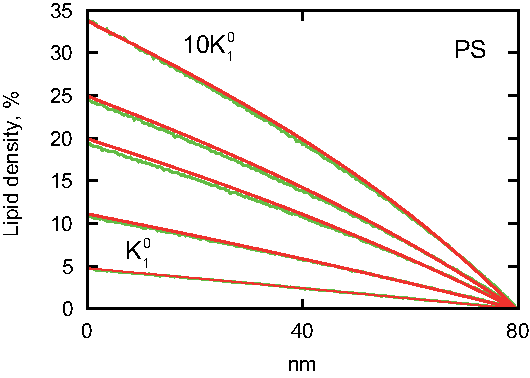
\includegraphics[scale=1.03]{../figures/single_grad_values_correction_half_lattice.pdf}

\caption[Comparison of the corrected CM with MCA for a single lipid gradient]{Comparison of the corrected CM \eqref{single_grad_correction}, $\gamma = 2$ (red line) with the MCA (green line) for a single lipid gradient. Gradients of monovalent PS lipids on binary PS/PC membrane for several LIIs: $K_1^0$, $2.5 K_1^0$, $5 K_1^0$, $6.7 K_1^0$ and $10 K_1^0$}
\label{fig:single_gradient_corrected}
\end{figure}

Fig. \ref{fig:single_gradient_corrected} shows the lipid profiles represented in Fig. \ref{fig:single_gradient}, B after the PS charge correction \eqref{single_grad_correction} with $\gamma=2$. For small gradients of PS (with less that 20\% peak value) the correction \eqref{single_grad_correction} does not significantly change the lipid profile. Note that even though the charge correction \eqref{single_grad_correction} is purely hypothetical and does not have any physical justification, it can efficiently resolve the strong coupling effect in the CM in binary PS/PC membrane systems.

\subsection{Lipid gradients on ternary membrane}

In this section I compare the two approaches in the case when the membrane system is ternary, i.e. consists of three types of lipids: PC, PS and PIP$_2$.
\begin{figure}[!ht]
\centering
  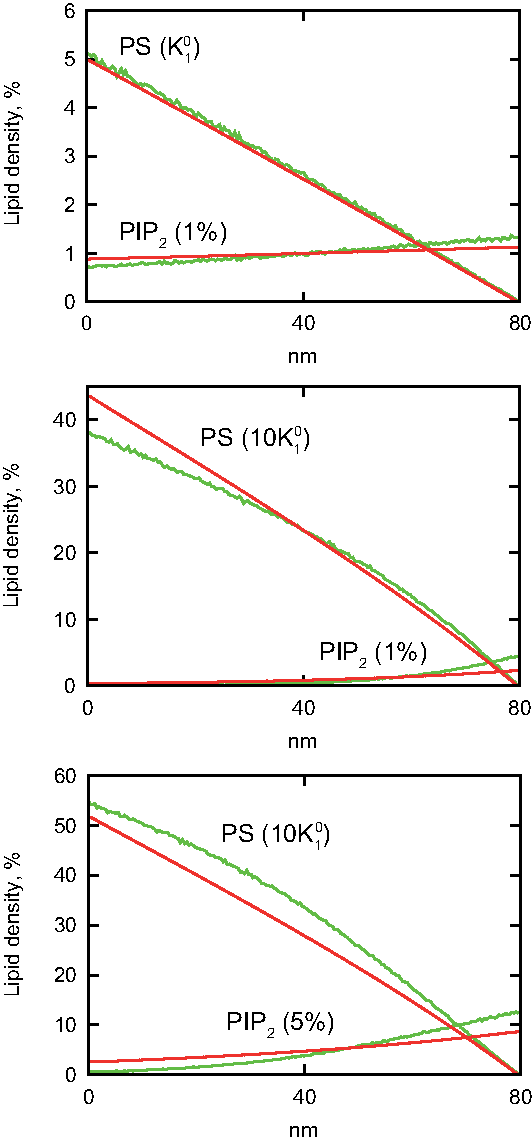
\includegraphics[scale=1.03]{../figures/double_grad1_half_lattice.pdf}

\caption[Comparison of CM with MCA for a ternary membrane with PS gradient]{Comparison of the CM (red line) with the MCA (green line) for a PS gradient on a ternary membrane. A, LII of PS is $K_1^0$ and initial uniform PIP$_2$ concentration is 1\%; B, LII of PS is $10 K_1^0$ and initial uniform PIP$_2$ concentration is 1\%; C, LII of PS is $10 K_1^0$ and initial uniform PIP$_2$ concentration is 5\%.}
\label{fig:double_grad1}
\end{figure}
I extend the CM to see how negatively charged lipids with different charges influence each other in the membrane. In this system there is always a gradient of one charged lipid species (PS or PIP$_2$) and another charged species has zero flux boundary conditions and responds to the gradient by changing its uniform profile.

I begin the comparison with low lipid concentrations and do not use the correction \eqref{single_grad_correction} for the charge of negatively charged lipids. In Fig. \ref{fig:double_grad1}, A, it is shown how a small gradient of PS lipids (with the LII $K_1^0$) change the profile of an initially uniform PIP$_2$. There is a small discrepancy in the PIP$_2$ profiles between the two models (Fig. \ref{fig:double_grad1}, A). This effect presumably appears due to the large negative charge of PIP$_2$ lipids, so that the system quickly reaches the strong coupling limit of electrostatic interactions ($\Sigma\sim q^3$).

Secondly, I compare the two models in the case of high PS gradient (with the LII 10$K_1^0$) (Fig. \ref{fig:double_grad1}, B). Note that due to the high PS gradient, PIP$_2$ lipids are completely displaced from the left boundary of the lattice, so that the PS gradient profiles on the left boundary are similar to the ones in the single PS gradient case (see Fig. \ref{fig:single_gradient}, B). At high PIP$_2$ initial uniform concentration of 5\% (see Fig. \ref{fig:double_grad1}, C) the discrepancy between the two models becomes larger, however, it is not surprising, since the value of $\Sigma$ in this case should be much higher than at the low PIP$_2$ concentration (Fig. \ref{fig:double_grad1}, A).
\begin{figure}[!ht]
\centering
  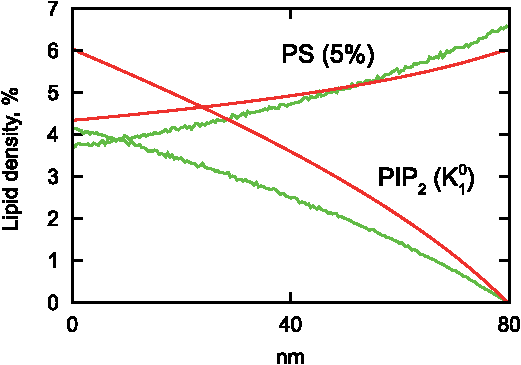
\includegraphics[scale=1.03]{../figures/double_grad2_half_lattice.pdf}

\caption[Comparison of CM with MCA for a ternary membrane with PIP$_2$ gradient]{Comparison of the CM (red line) with the MCA (green line) for a  with PIP$_2$ gradient on a ternary membrane. LII of PIP$_2$ is $K_1^0$ and initial uniform PS concentration is 5\%;}
\label{fig:double_grad2}
\end{figure}

Finally, I investigate a reversed situation when a gradient of PIP$_2$ lipids influences a uniform profile of PS lipids (Fig. \ref{fig:double_grad2}). Since biologically relevant PIP$_2$ concentrations do not exceed at most 10\%, I use a small value of PIP$_2$ LII ($K_1^0$).


Figs. \ref{fig:double_grad1} and \ref{fig:double_grad2} show that, presumably in the mean field approximation used in the CM model, the contribution of multivalent PIP$_2$ molecules to the electrostatic potential is slightly underestimated. However, quantitatively (trends and functional dependencies) the two models are in a very good agreement.

\subsection{Distribution profiles of PLCs on binary membrane}

Having compared the CM and the MCA approaches in membrane systems with lipid gradients, it is also important to compare them in the presence of the Lys-5 peptide species. For this configuration in the MCA the probability distributions of the peptide on the membrane are calculated as described in section \ref{new_MCA_description}. Concentrations of PLCs in the CM model are calculated for zero-flux boundary conditions. Lipid boundary conditions are the same as in subsection \ref{chap:single_gradient}. Diffusion coefficients of PLCs are chosen to be identical and equal to $D_p^0$ = 1 $\mu$m$^2$/s (the maximal lipid diffusion coefficient $D_L$, see subsection \ref{testing_calibration_MCA}).

\begin{figure}[!ht]
\centering
  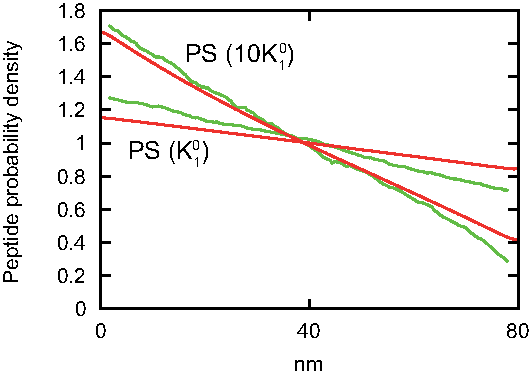
\includegraphics[scale=1.03]{../figures/peptide_grad1.pdf}

\caption[Comparison of CM and MCA for peptide probability distributions]{Comparison of peptide probability distributions for the MC (green line) and the CM (red line) for two LIIs of PS: $K_1^0$ and $10 K_1^0$.}
\label{fig:peptide_grad1}
\end{figure}

Fig. \ref{fig:peptide_grad1} shows the comparison between the PLCs profiles in the CM and in the MCA for two lipid gradients (corresponding to $K_1^0$ and $10K_1^0$ LIIs). In the MCA, in agreement with the hypothetical peptide drift mechanism, described in chapter \ref{non_uniform_membrane}, in the case of the large PS gradient the peptide significantly accumulates on the left membrane boundary with the peak value corresponds to $\sim$1.7 times increase in the peptide concentration. For the small lipid gradient the increase is about 1.3 times. The CM model is in a very good quantitative agreement with the MCA results. The negligible discrepancy between the two models can be corrected by varying of the PLCs diffusion coefficient. For example, if one assumes that complexes with a small number of bound PS lipids are faster than heavy complexes that are fully occupied by PS lipids, so that their diffusion coefficients are corrected as follows:
\begin{align}
\label{peptide_correction}
 D_{0,0} &= 1.3\cdot D_p^0 \nonumber \\
 D_{0,1} &= 1.2\cdot D_p^0 \nonumber \\
 D_{0,2} &= 1.1\cdot D_p^0
\end{align}
the peptide probability distribution profiles in the CM become almost identical to the ones in the MCA (Fig. \ref{fig:peptide_grad2}).

\begin{figure}[!ht]
\centering
  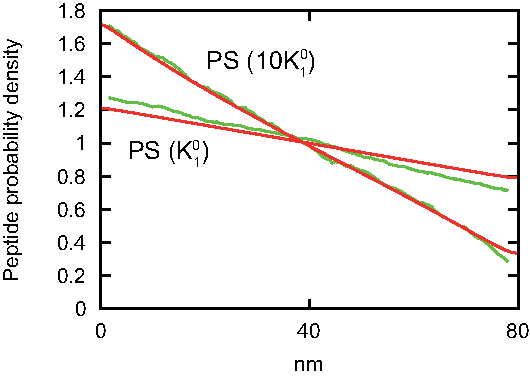
\includegraphics[scale=1.03]{../figures/peptide_grad2.pdf}

\caption[Comparison of the corrected CM and MCA for peptide probability distributions]{Comparison of peptide probability distributions for the MC (green line) and the corrected \eqref{peptide_correction} CM (red line) for two LIIs of PS: $K_1^0$ and $10 K_1^0$.}
\label{fig:peptide_grad2}
\end{figure}

Based on the comparison of the CM with the MCA, one can conclude that the constructed CM faithfully describes the lateral dynamics of the lipids and the peptides on the cell membrane under the action of electrostatic forces.